\section{CICIDS2017 Is Near-Degenerate}
\label{sec:degeneracy}
% Budget: 0.75 page. Source: DECISIONS.md s10, s15, s16; results/phase0/cicids/nn_by_family.csv,
% grid_sweep.csv.
% - Every family with >500 eval rows, and benign, sits far below the leakage threshold at every
%   dedup grid and with burst splitting.
% - Consequence: no learning claim on CICIDS; S0 learning claim made on synthetic instead.
% - The 94% of benign validation rows discarded for an honest threshold (s23).
% TODO: prose.

\begin{figure}[t]
  \centering
  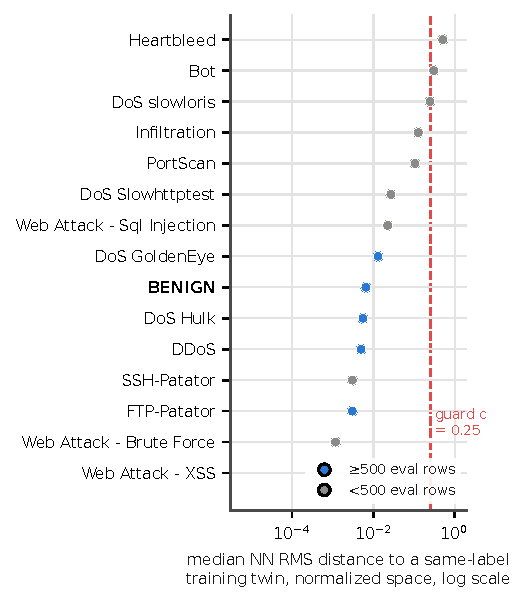
\includegraphics[width=\linewidth]{figures/F2_nn_by_family.pdf}
  % Source: results/phase0/cicids/nn_by_family.csv + leakage_report.json (benign row).
  % Regenerated by: python scripts/run.py figures --only F2  (experiments/paper_figures.py:fig_f2)
  \caption{TODO caption. Per-family median nearest-neighbour RMS distance to a same-label
  training twin (log scale); families with fewer than 500 trusted\_eval rows greyed out as
  not reportable. Dashed line: the guard-(c) leakage threshold, 0.25.}
  \label{fig:f2-nn-by-family}
\end{figure}
